\documentclass{ltjbook}
\usepackage{docmute}
\usepackage{../../myStyle}

\begin{document}
\VerbatimFootnotes

\chapter{3つめの推定法}
\label{ch25_bayesian_intro}

ここまで尤度を使った推定方法について説明してきました。モーメント法と最尤法，平均値についてはいずれも同じ答えが出るのですがその考え方が違うというところを確認してきましたね。さてここからは，もう1つの推定法である\keytermL{ベイズ法}{べいずほう}について解説します。そのためには，ベイズ法の根本的な法則について知っておいた方が良いので，少し回りくどいかもしれませんが，まずはそこから説明していきましょう。目的を先に教えてくれないとやだよ，という人のために一言で目的だけ言っておきます。ベイズ法は最尤法と同じく確率モデルを使うのですが，尤度が「確率じゃない」という妙な性質があったのに対し，ベイズ法は答えを確率で出します。尤度を確率にするための仕掛けがこれから始まるのです。
\section{ベイズの定理}
ベイズというのは人の名前で，トーマス・ベイズ(Thomas Bayes，1702年 - 1761年4月17日)はイギリスの長老派の牧師であり数学者でもある人です。この人の考えた「逆確率の法則」から端を発した推定法が，21世紀の現代においてとても重要なものになってきています。ベイズ牧師の考えついた法則は非常に単純なもので，簡単に書くと次のような式で表現できます。
\[ P(A|B) = \frac{P(B|A)P(A)}{P(B)} \]

この式の意味するところを，確率の用語をいろいろ紹介しながら説明していきたいと思います。

話をわかりやすくするために，具体的な数値例とともに話を進めましょう。
たとえば，ある学校の生徒数は男子が40人，女子が60人だったとします。そこからランダムに一人を選び出した時，それが男子である確率はどれぐらいでしょうか？ この確率を$P(\mbox{男子})$とすると，
\[P(\mbox{男子})=\frac{40}{100}=0.4 \]
であることはすぐにわかりますね。

では次に\keyterm{同時確率}{どうじかくりつ}{joint probability}という考え方を導入しましょう。これは先ほどの学校について，表\ref{tbl::25_02}のように学年情報を追加した例を使って説明します。

\begin{table}[ht]
	\centering
	\caption{ある学校の学年と性別のデータ}
	\begin{tabular}{rrrrr}
		\hline
		   & 1年 & 2年 & 3年 & 合計  \\
		\hline
		男子 & 15 & 12 & 13 & 40  \\
		女子 & 22 & 20 & 18 & 60  \\\hline
		合計 & 37 & 32 & 31 & 100 \\\hline
	\end{tabular}
	\label{tbl::25_02}
\end{table}

記号で表現するために，性別の変数をAとし，$A_1=$男子，$A_2=$女子，学年の変数をBとして$B_1=$1年生，$B_2=$2年生，$B_3=$3年生とします。

ここでランダムに一人を選び出した時，それが「3年男子」である確率はどれぐらいでしょうか？ これは「性別は男」かつ「学年は3」なので，性別と学年の両方の条件が入った同時確率といい，$P(A_i,B_j)$と書きます。これは表から，次のように計算できますね。
\[ P(A_1,B_3)= \frac{13}{100}=0.13 \]

次に用語として\keyterm{周辺確率}{しゅうへんかくりつ}{marginal probability}というのを考えます。これはある分割に関してすべて足し上げたもの，というものですが，要するに表\ref{tbl::25_02}の合計欄のことです。たとえば「男子生徒についての周辺確率」は，男子生徒が学年によって3つに分割されていますが，これをすべて足し上げるので，1年男子+2年男子+3年男子で求まるものです。
式で言うと，次のような意味になります。

\[ \sum_{j=1}^3 p(A_i,B_j) = p(A_i) \]
\[ \sum_{i=1}^2 p(A_i,B_j) = p(B_j) \]

全部の数字を足し合わせるので，その変数の確率の話ではなくなる，と思ってください。このように一方の変数のすべての確率を足し合わせることを\textbf{周辺化}する，といいます。

では次のステップ。今度は\keyterm{条件つき確率}{じょうけんつきかくりつ}{conditional probability}というのを導入します。無作為に学生を選び出す時，「選ばれたのが女子である」ということが先にわかったとします\footnote{たとえば名前とか容易に類推できた，といったようなシーンです。最近では名前だけから性別を判断するのは難しくなりましたが，かつての名残で明らかにわかるような名前だったと思ってください。}。その時，その生徒が2年生である確率はどれくらいでしょうか？ この問いを「女子という条件がついた上での確率」という意味で，条件つき確率といい，表現としては$P(\mbox{2年生}|\mbox{女子})$と書きます。2つの分割を縦棒で区切り，条件の方が後ろに書きます。「女子という条件が与えられた上での二年生の確率は」というように読んだりします。

ちょっと状況はややこしくなりましたが，確率の計算そのものはそれほど難しくありませんね。女子である，というのが決まっているので，分母が変わるだけなのです。つまり，
\[P(B_2|A_2)=\frac{20}{60}=0.333... \]
となります。

条件つき確率の計算は分母が変わったと思えばいいのですね。この条件つき確率は，同時確率を周辺確率で割っても計算できます。すなわち，
\[ P(B_2|A_2) = \frac{P(A_2,B_2)}{P(A_2)}=\frac{0.2}{0.6}=0.333... \]
となるわけです。

今度は学年が一年生の時，二年生の時，三年生の時，で考えてみましょう。この場合，それぞれで分母が変わりますし，条件付き確率も変化します。性別が変わると学年の確率が変わりますし，学年が変わると性別の確率も変わります。このような関係にあるので，この性別と学年という2つの変数は関係しあっていることがわかります。逆に，一方の変数が変わっても他方の変数に影響しない場合，両者は\keyterm{独立}{どくりつ}{independent}だ，といいます。
確率において独立であるとは，すべての$i,j,k$において次の関係が成り立つことを言います。

\[ p(A_i|B_j) = p(A_i|B_k) \]

これまでも(確率的に)独立である例の話はいろいろしてきました。たとえばコイントスを続けて行うときは，それぞれの試行は独立だよね，という話をしました($\to$セクション\ref{iidexample}，Pp.\pageref{iidexample})。1回のコイントスの結果が次のコイントスの結果に影響しない，という意味です\footnote{逆に一回のコイントスが次のコイントスに影響するとはどういうシーンでしょうか? 無理矢理考えるなら，コインが意思を持って「さっき表になったから，次は裏にしようとする」とか，トスしたコインを受け取り損ねて地面に落下し，片方の面が欠けて他方の面が出やすくなった，というようなシーンです。コインは意思を持ってないし，硬いものですから，これらはやはり考えにくい話ですよね。}。

ここで独立しているのならば，ここまでの式展開から，

\begin{equation}
	\begin{array}{lll}
		p(A_i|B_j)               & = & p(A_i|B_k)                \\
		                          &   &                           \\
		\frac{p(A_i,B_j)}{p(B_j)} & = & \frac{p(A_i,B_k)}{p(B_k)} \\
		                          &   &                           \\
		p(A_i,B_j)p(B_k)          & = & p(A_i,B_k)p(B_j)
	\end{array}
\end{equation}
ここですべての$k$の状態について$B_k$を数え上げる，つまりBを周辺化します。
\begin{equation}
	\begin{array}{lll}
		p(A_i,B_j)\sum_{k=1}^K p(B_k) & = & p(B_j)\sum_{k=1}^K p(A_i,B_k) \\
		                              &   &                               \\
		p(A_i,B_j)                    & = & p(B_j)p(A_i)
	\end{array}
\end{equation}

ここからわかるように，AとBが独立である場合は，同時確率と確率の積がおなじになります。独立している事象が起こる確率は，それぞれの確率を掛け合わせましょうということです。これまでも，コイントスやサイコロの例で，2回続けて計算する場合はその積で表現してきましたよね。
確率$\theta$で表が出るコインで，2回続けて表が出る場合は$\theta \times \theta=\theta^2$，表・裏と出る場合は$\theta \times (1-\theta)$といった表現をしてきました。
独立した事象は掛け算で表せる，というのはこういう理屈からなんですね。


さて，これで用語の準備は終了です。ここから式の展開が面白くなってきます。

あらためて，条件付き確率は同時確率を周辺確率で割ったもの，でしたね。つまり，
\[ P(B_j | A_i) = \frac{P(B_j,A_i)}{P(A_i)} \]
ここで右辺の分母を両辺にかけて，
\[ P(A_i)P(B_j|A_i) = P(B_j,A_i) \]
とします。これはA,Bが何であるかにかかわらず，一般的に成立します。たとえば$P(A_i|B_j)$と記号をひっくり返しても，
\[ P(A_i|B_j) = \frac{P(A_i,B_j)}{P(B_j)} \]
より
\[P(B_j)P(A_i|B_j) = P(A_i,B_j) \]
としても構いませんね。


ところで，「2年の男子」と「男子の2年」というのは同じ意味です。つまり，
\[P(B_j,A_i) = P(A_i, B_j) \]
ですから，上の式をつなぎ合わせて
\[P(A_i)P(B_j|A_i) = P(B_j)P(A_i|B_j) \]
とできます。ここで両辺を$P(B_j)$で割って清書すると，
\[ P(A_i | B_j )=\frac{P(B_j|A_i)P(A_i)}{P(B_j)} \]
が得られます。やったね！ベイズの定理が導出できました。


さて，これの何がすごいのでしょう？ 数式を「記号の羅列だ！」と思って拒否するのではなく，その意味をしっかり味わってみましょう。
\section{ベイズの定理の意味}
\subsection{因果の向きについて}
さてベイズの定理のすごいところは，左辺と右辺の中にある条件つき確率の中身が\textbf{ひっくり返っているところ}にあります。
これがひっくり返ると何がうれしいのでしょうか。
ベイズの定理の左辺には$P(A|B)$があり，右辺は分子に$P(B|A)$を含んでいます。$P(A)$(分子の2つ目の項目)や$P(B)$(分母)のことはいったん忘れてくれてもいいですし，
\[ P(A|B) = P(B|A) \times \frac{P(A)}{P(B)}\]
と考えて，$P(A|B)$が$P(B|A)$の関数である，と読み取ってくれても構いません。

ここでAを「心のモデル」，Bを「データ」と考えてみてください。
私たちは心の仕組みを考える時に，モデルをたてます。「あの人がAという行動をとったのは，心の状態がXだったからではないか」というのは心というモデルを立てて考えるということなのでした。心の状態がXであれば，人はAという行動をとるであろう，というのが研究者の仮説，モデルなのです。つまり，$P(\mbox{データ}|\mbox{モデル})$が心理学でやっていることなのです。

ところが実際には，手に入れることができるのはデータだけです。心がどうなっているかはわかりませんが，人が$\diamond\diamond\diamond\diamond$な行動をとった，という事実だけがそこにあるのです。この事実を使って，我々のモデルがどれぐらい正しいのか。あるいはモデルのパラメータはどうなっているのか，を検証したいわけです。つまり，研究の営みとは$P(\mbox{モデル}|\mbox{データ})$であり，データを所与(条件)としたときの，モデルの確率を考えることなのです。データをとってモデルを検証するという営みが成り立つ根拠を，ベイズの定理が示してくれていると言えるかもしれません。大事なのは，不確かな状況においては我々は確率的にしか判断をできず，ベイズの定理では条件の向きをひっくり返して計算できる，という点です。原因が結果を引き起こす確率が知りたい時に，結果を手にすることで，原因がどれほどあり得たかを考えることができる。それがベイズの定理のポイントなのです。ベイズの定理は因果の向きを逆にできる，ということを示しているので，\keytermL{逆確率の法則}{ぎゃくかくりつのほうそく}と呼ばれることもあります\footnote{ベイズ自身がこの法則を発見した時に，「なんかおかしなことになってるかも」と思って結果を公表しなかったと言われています。神様が決めた世界を裏返しにすることに，背徳感のようなものを感じたのかもしれません。}。

\subsection{確率という数字，再考}
ここまでベイズの定理の説明は，性別や学年など離散的な数字をもとに説明してきましたが，連続的な確率変数でも成り立ちます。連続的な確率変数の場合，すべての確率を足し合わせるという操作が積分することに変わりますが，それ以外は本質的に変わりません。一般的に書くと，

\[ f(\bm{\theta}|\bm{x}) = \frac{f(\bm{x}|\bm{\theta})f(\bm{\theta})}{f(\bm{x})} \]

となります。ここで$\bm{\theta}$はパラメータで，複数ある場合があるのでベクトルの表記(太字)にしてあります。$\bm{x}$はデータのことで，これも1つのデータではないので太字にしています。$f$は連続的な確率関数だと思ってください。
先ほど説明したように，この関数は

\[ f(\bm{\theta}|\bm{x}) = f(\bm{x}|\bm{\theta}) \times \frac{f(\bm{\theta})}{f(\bm{x})} \]

と考えても構いません。ここで$f(\bm{x}|\bm{\theta})$は，パラメータが所与の元でのデータの出てくる確率ですから，\keytermL{尤度}{ゆうど}だ，ということがわかります。式の左辺は$ f(\bm{\theta}|\bm{x})$ですから，データが所与の時のパラメータの確率ですね。これをとくに\keyterm{事後確率}{じごかくりつ}{posterior probability}と言い，それに対して右辺の$f(\bm{\theta})$は\keyterm{事前確率}{じぜんかくりつ}{prior probability}といいます。
ベイズの式は，確率を確率に変換する公式なのです。

ところでこの\keytermL{確率}{かくりつ}って何なのでしょうね。パラメータについての事前の確率とは，一体どういう意味があるのでしょうか。

さて，確率の公理を思い出してほしいのですが，確率とは次の条件を満たす数字だということでした。
\begin{enumerate}
	\item 確率の値は非負(正または0の数字)
	\item 全標本空間におけるすべての事象の確率の合計は1.0
	\item 任意の2つの相互に排他的な事象について，どちらか一方が発生する確率は個々の確率の和である
\end{enumerate}
そして，確率には\keytermL{頻度主義}{ひんどしゅぎ}的な考え方と，\keytermL{主観確率}{しゅかんかくりつ}という考え方があって，どちらでもこの公理を満たしている限り確率として計算できます，という話をしてきました。

高校数学までは頻度主義的な意味で確率が説明されてきたと思います。すなわち，コインやサイコロを\textbf{無限に}投げ続けると，パラメータの値は1/2や1/6に近づいていくだろう，ということです。この無限に繰り返すと1つの値に収束するというのは，確率的収束という数学的な証明がされる考え方ですが，現実には無限に行うというのはあり得ません。心理学の実験も，同じ実験を無限に繰り返すと，という設定のもとで考えて帰無仮説検定を行ったりしますが，それがそもそもあり得ない前提じゃないか，と言われたらどうしようもないのです\footnote{さらに帰無仮説というあり得ない仮定を置いてますから，一体どこの世界の話をしているのやら，という気持ちになります。}。無限の回数を考えて，その相対頻度，割合で確率を考えるので\keytermL{頻度主義}{ひんどしゅぎ}と呼ばれています。

これに対して天気予報などは，信念の確からしさを確率で表現しています。明日晴れる確率が30\%というのは，明日という日が無限に繰り返されればそのうちの3割は晴れている，と言うのはやはりおかしいわけです。どんなループに巻き込まれてしまったのでしょうか，明日が無限に繰り返されるなんて！
そういう意味では，普段私たちが慣れ親しんでいるのは，自分達の確信の強さ，どの程度その事象を信じているかと言う信念の強さを表している数字と言えます。明日100\%雨が降る，というのは完全にその状態を信じているということですし，50\%の降水確率は雨が降る可能性が半分，降らない可能性が半分だと考えていると言うことですね。また，相対頻度・割合で考えるときは，全体で割った平均的な数字を出すことになります。この頻度主義的な考え方ですと，たとえば野球のシーズン最初の試合，勝ったチームは勝率100\%になります。一試合しかしていないので，1/1だからです。でも誰も「このチームは今シーズン一度も負けないだろう」と本気で信じているわけではないですよね。あるいは最初の打席でヒットが出なかったからといって，打率0割，永遠に打てない打者だとは誰も考えません。本当はもう少し低い勝率，高い打率だと思っているのに，そう表現できていないのです。その意味では，「確からしさを表す数字」として確率を使うほうが自然かもしれません。

つまり，確率という数字の見方には大別して二種類あるということです。どちらが正しいとか，どちらが優れているというわけではありません。どちらも上に述べた3つの公理を満たすものですから，確率は確率なのです\footnote{というか，この公理はさまざまな確率の考え方の共通基盤・最低限のルールをまとめただけなので，必然的にどちらにも合うようになっているというだけです。}\footnote{ちなみに，主観確率が成り立つためにはどのような条件が必要かということについては，\textcite{Gilboa2014}などに詳しく論じられています。また\textcite{shigemasu2019}は主観確率という確率が成立する条件として，1.すべての不確かな事象の蓋然性は相互に比較できる，2.蓋然性に関する判断は相互に矛盾しない，3.まったく可能性がない状態を0，確実に起こることを1として，0から1までのすべての数値を取りうる不確定な状態を作る実験が存在する，の3つを挙げています。人間が必ずこのルールに則って判断している，という話ではなく合理的な判断があるとするならば，この規則に則っていると考えるべきであるという規範理論であり，「そんな状況はあり得ないからだめだ」というのは反論として的外れなものです。経済学では合理的に価値判断をする人間を仮定して理論を組み立てており，この不確実状況下での意思決定論もそれと同じ系譜，かつ，ベイズ統計学の応用を許す理論的基礎になっているといえるでしょう。}。

頻度「主義」とか「主観」確率，という言葉の使い方をすると，個人の考え方で数学のルールや数字の意味が変わるのはおかしい，と思う人がいるかもしれません。数学のルールは人類が存在しなくても永遠普遍の真実だ！という考え方があるのもわかります。主義や信念の対立で優劣を決めたいわけではないのですが，頻度主義的な発想とベイズ主義的な発想とでは，母数についての考え方が違っているのも事実です。頻度主義的な発想では，無限に試行を繰り返せばいつかは答えにたどり着くはずで，言い換えれば「真実はいつも1つ」なわけです。ただそれが直接わかり得ないから，徐々に近づいていくしかない。図\ref{fig:25_06}の上の段にあるように毎回の試行で信頼区間をとって表現できますが，これは本当の値(図では0.5が真の値としています)を跨いでいるかどうか0/1の判定が続くわけです。

これに対して主観確率で考えるベイズ法による推定は，そもそも母数の値がわかりませんので，わからないことを確率で表現する。最初は幅の広い，全域に渡るような確率でぼんやり考えるのです。これに毎回の試行＝データを積み重ねることによって，この幅を狭めていき，「この辺にあるんじゃないかなあ」という確信度を高めていくという考え方です。
\begin{figure}[ht]
	\centering
	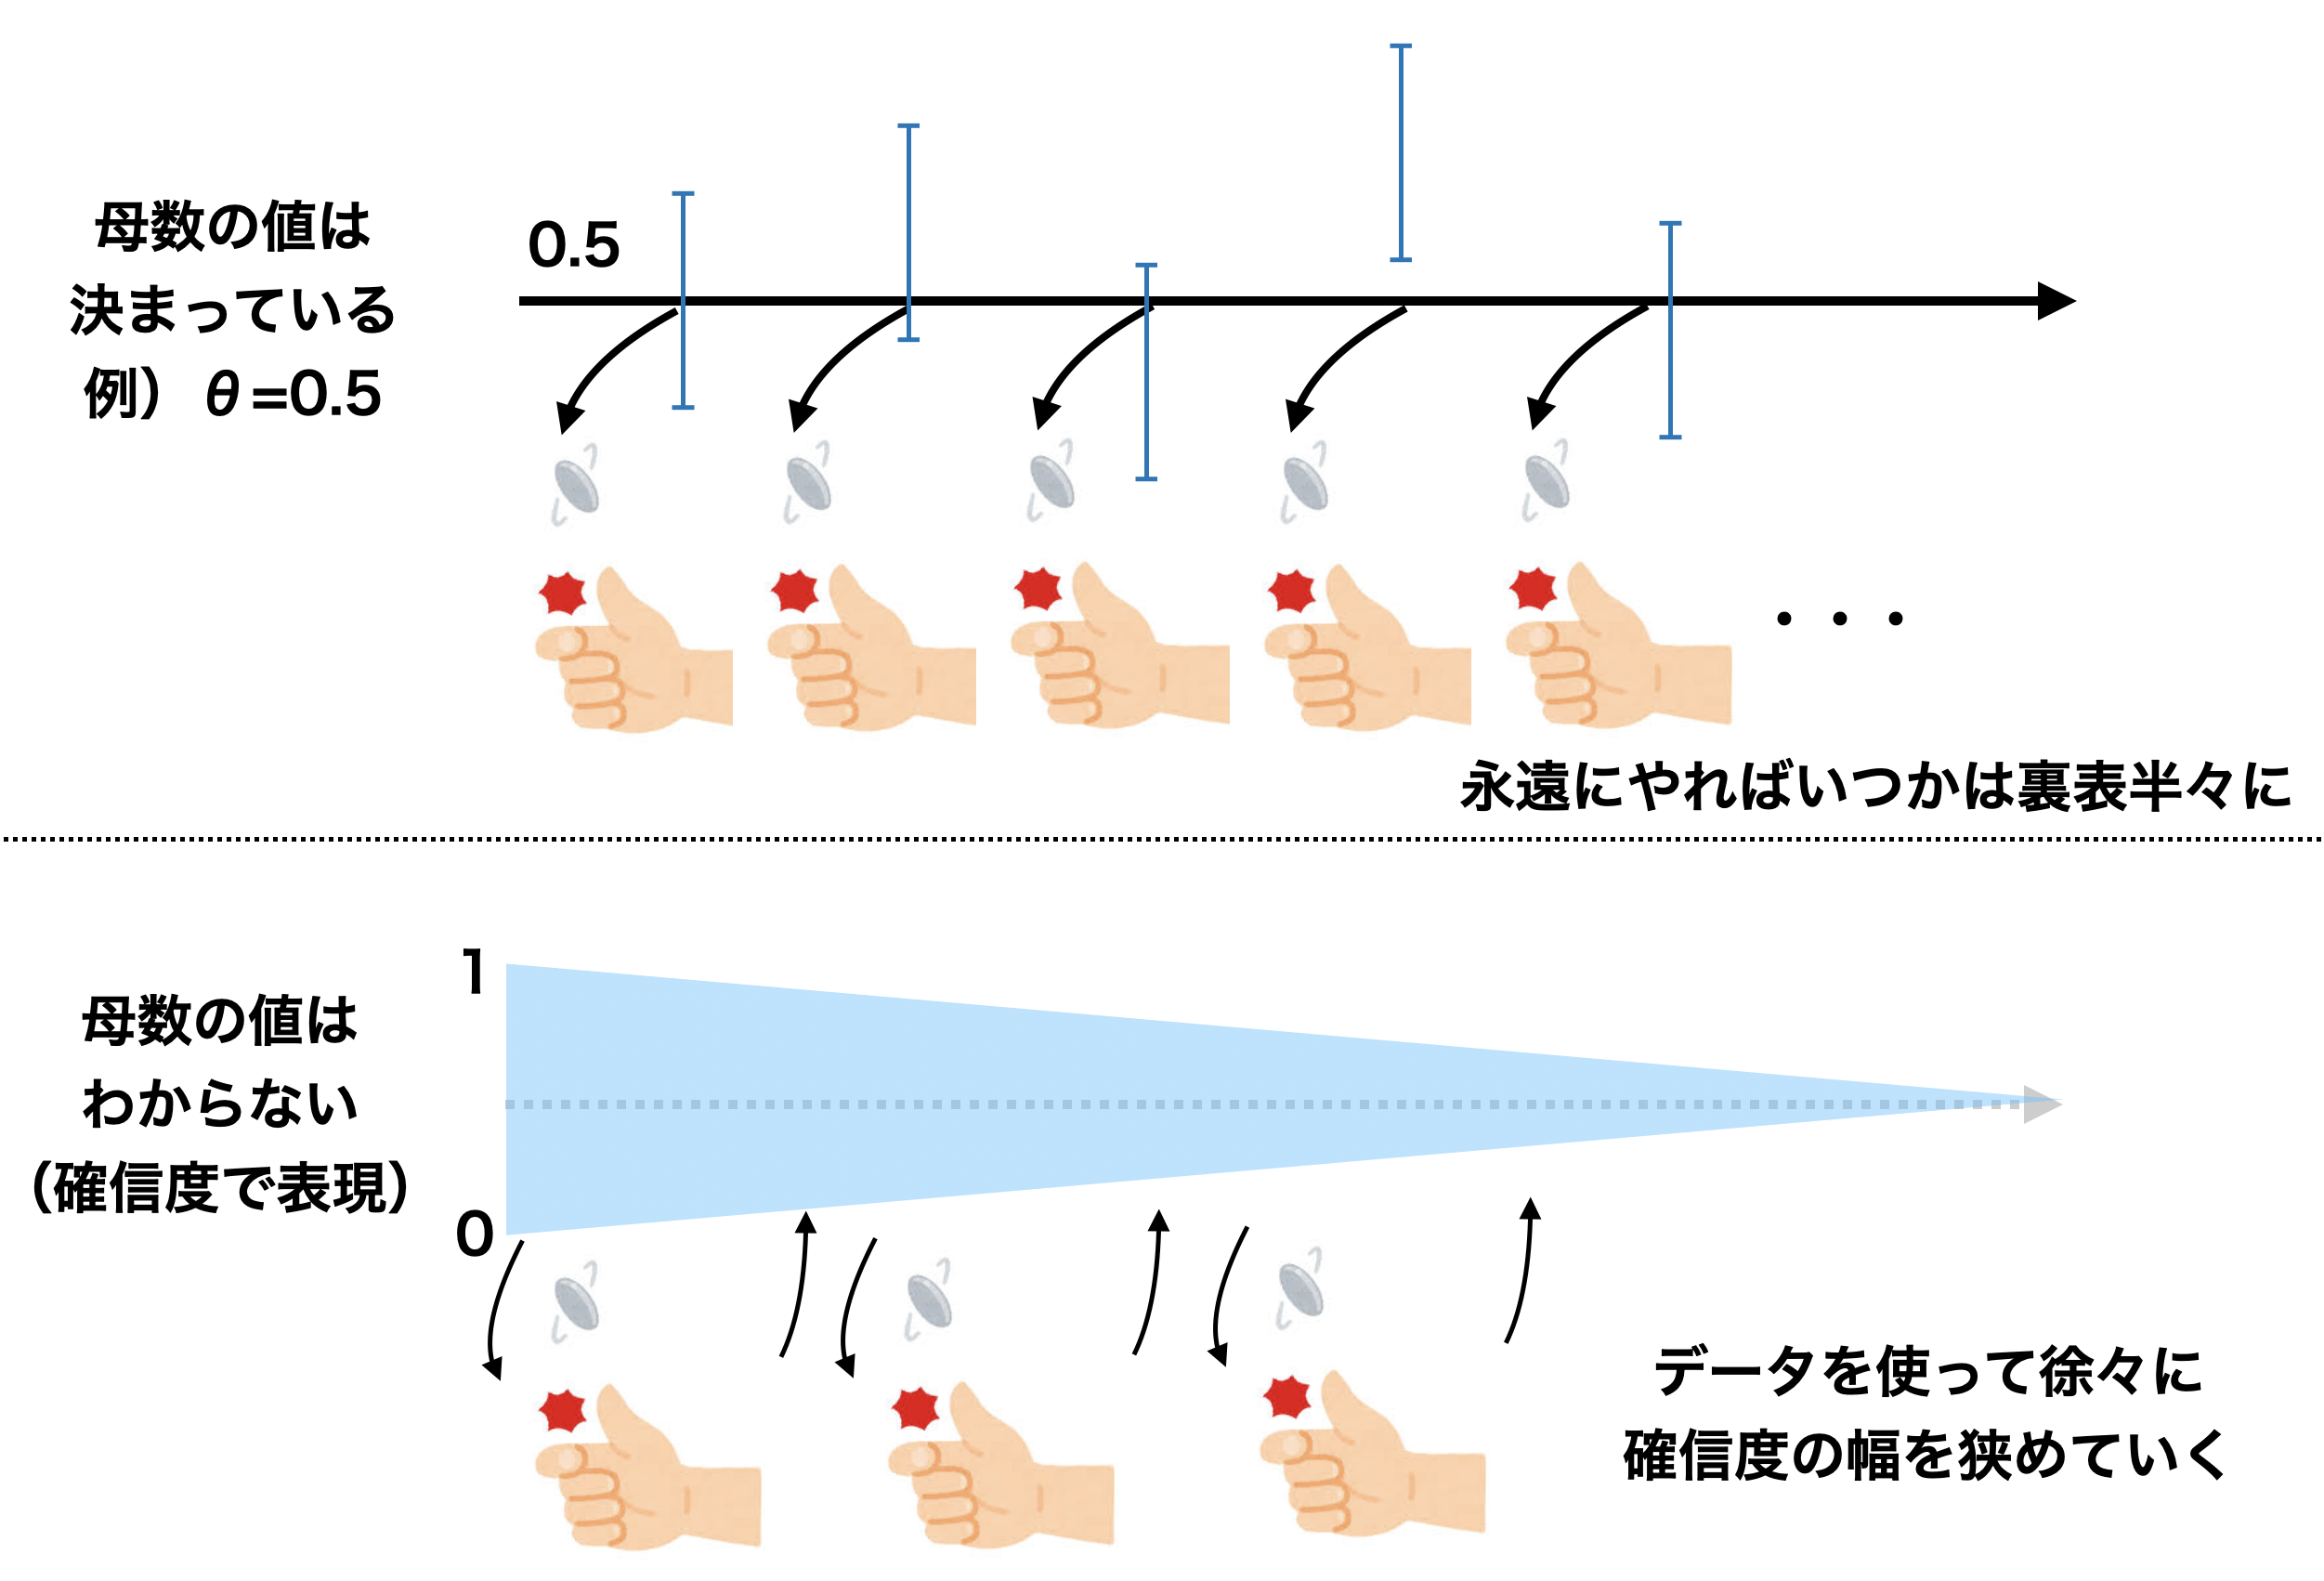
\includegraphics[keepaspectratio,width=0.8\linewidth]{figures/25_bayesian_intro/two_types_probability.png}
	\caption{確率についての2つの考え方}
	\label{fig:25_06}
\end{figure}

この後，ベイズ法による推定を説明していきますが，このとき真の値が定数としてただ1つ定まっている，と考えられるかどうかについては，とくに定まりがありません。母数は定数で定まっている，ただそれが確率的にしかわからないだけだという考え方をするのか，母数がそもそも確率的に分布していると考えるのか，いずれの考えであってもいいでしょう\footnote{このような考え方の違いは，量子力学のコペンハーゲン解釈，ボーアとアインシュタインの哲学の違いに似たところがあります。アインシュタインは「神はサイコロをふらない」といい，物理現象は確たるものがあると信じていました。これに対してボーア率いるコペンハーゲン学派の解釈は，物理現象は究極的に確率的に存在していると言い，シュレディンガーの猫も生と死の重ね合わせた状態である(観測するまでわからない)と言い切るわけです。現代物理学としては量子力学が優勢ですが，アインシュタインの気持ちもわかりますね。}\footnote{ベイズ統計の中にもさまざまな流派があり，Twitterでは時折喧嘩になっています。争点はこの「主観確率」を認めるかどうかというところで，「人間はすべての情報を手に入れることはできないので，自分の知り得た情報の範囲の中で最適な判断をするしかない。」と考える主観ベイズ派と，「手に入れた情報はなんらかの確率分布から生成されたサンプルに過ぎず，確率的に変動するサンプルから真の分布の状態を推論するのだ」という情報統計学的立場があります。後者は日本の数理統計学者(赤池弘次，渡辺澄夫)が展開している議論で，AICやWAICなど有用な指標を提案していることもあって，日本ではよく知られています。しかし主観ベイズ派は，古くからいかにして主観的確率判断が成り立つかについて緻密な理論を打ち立てており，世界的にはこちらの方が多数派かもしれません。}。

現代的に，あるいは統計のユーザとしてはプラグマティックに「使い物になるほうが正しい考え方だ」という割り切り方をしても良いでしょう。いずれにせよ，これらの手法によって表現されるものの意味の違いについて，少し注意しておいていただければと思います。

\section{3つの推定方法の比較}

さて，これで\keytermL{モーメント法}{もーめんとほう}，\keytermL{最尤法}{さいゆうほう}，\keytermL{ベイズ法}{べいずほう}という3つの推定方法が出そろったことになります。それぞれの特徴について，今一度確認しておきましょう。

\paragraph{モーメント法}
最初に説明したのは，標本平均をつかって母平均の推定値とする，不偏分散をつかって母分散の推定値とする，という，記述統計量に密着した推定法，モーメント法でした。

図\ref{fig:25_02}がそのイメージです。母集団から標本を得ている図ですが，まず母集団で実際にどのような分布になっているかは分かりません。図では薄い黒で描かれているのが神の目でみた母集団の分布です。我々はこれについては知り得ないので，正規分布じゃないかな，という仮定を置くわけです。正規分布は位置と幅，平均と標準偏差をパラメタに持ちますから，これが推定したい母数。この分布から無作為に標本が得られたとすると，小サンプルからなるヒストグラムが描けます。標本は正規分布かと言われると，サンプルサイズが小さい場合はとてもそうは思えませんが，原理的には正規分布に従っているはず。そして標本平均は母平均の，不偏分散は母分散の推定値として使えるということが数理統計学によって証明されているので，この標本統計量を母数を推定するための値として使う，というのがモーメント法です。ここには標本をたくさん集めれば，いずれは1つの値に収束していくという，無限試行の極限として確率を定義する考え方，いわゆる頻度主義的な考え方が根底にあります。

\begin{figure}[ht]
	\centering
	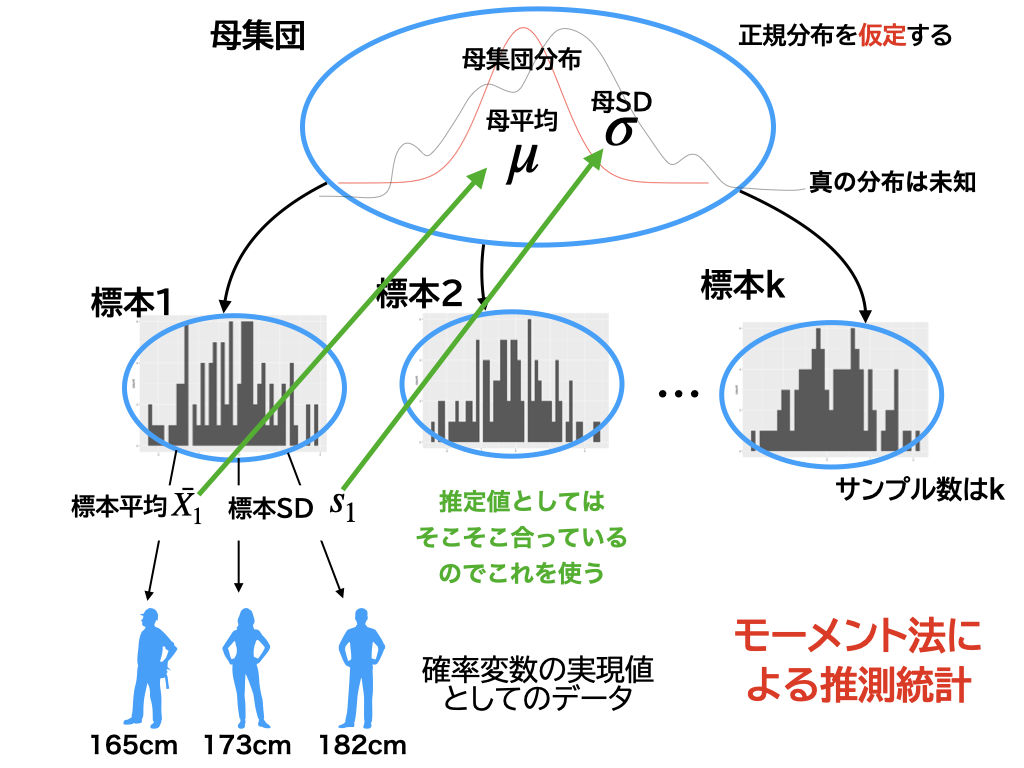
\includegraphics[keepaspectratio,width=0.8\linewidth]{figures/25_bayesian_intro/method1_moment.png}
	\caption{モーメント法による母数の推定}
	\label{fig:25_02}
\end{figure}

モーメント法は古くから使われてきた手法であり，また手続きのパターンが決まっているので統計パッケージに採用されやすく，最も広く普及した方法といえます。今でも心理統計のテキストのほとんどが，モーメント法に依拠しています。帰無仮説検定は基本的にこの系譜にあり，心理学においても他の分野においても，長らく使われてきています。ただし手続きがパターン化，悪く言えばマニュアル化し，「これさえやっておけば良いだろう」という使われ方が，マニュアルの誤読や誤解，ルール違反を生み出すことにもなりました\footnote{これはこの統計手法が悪いというのではなく，何でもルール化してしまうと同時にハックする方法もできてしまうということですので，研究に対する態度の問題です。}。

ただし，マニュアル自体もアップデートされていってます。帰無仮説検定を行うには，結果を後から改竄したと言われないで済むように，事前のサンプルサイズ設計，検定基準の設定を行う。どこからどこまでが計画の範囲で，どこからは探索的な分析であるかといったことを明確にしておく。これらを事前に登録・公開しておくといったことが推奨されるようになっています。「とりあえず取れるだけデータを取って，あとでいろいろ分析してみよう」というやり方は，探索的な研究領域では有効かもしれませんが，帰無仮説検定の手続きには向いていないということです。かつてはそのような実践がスタンダードでしたが，近年はそうもいかないということです\footnote{これは昔は適当に運用されていたが，最近はコンプライアンス意識が高くなって息苦しくなってきた，というような話とは違います。まず昔のマニュアルが作られた頃に比べて，計算機の能力が段違いです。かつては$p$値をパソコンで厳格に出すことすらむずかしかったわけですから。加えてもちろん，再現性問題\parencite{Ikeda2016}があります。心理学の研究が再現されない原因の一つに，統計の誤用悪用，問題ある研究実践(QRPs)があったということ。これらの反省にたって，自浄作用として生まれてきたムーブが事前登録などの対策なのです。真面目に学問をやる上では大事なことです。}。

\paragraph{最尤法}
さて，第二に，確率分布関数をつかってそれに合うパラメータを探すという，最尤法という考え方もあります。(図\ref{fig:25_03})。これは分散分析の生みの親，R.A.フィッシャー先生が考えた方法で，データが正規分布する母集団から生成されている，という情報をヒントに，データが与えられた時のパラメータがありそうな場所を探す方法，手元のデータが最も出てきやすいパラメータは何かを考える，という方法でした。
\begin{figure}[ht]
	\centering
	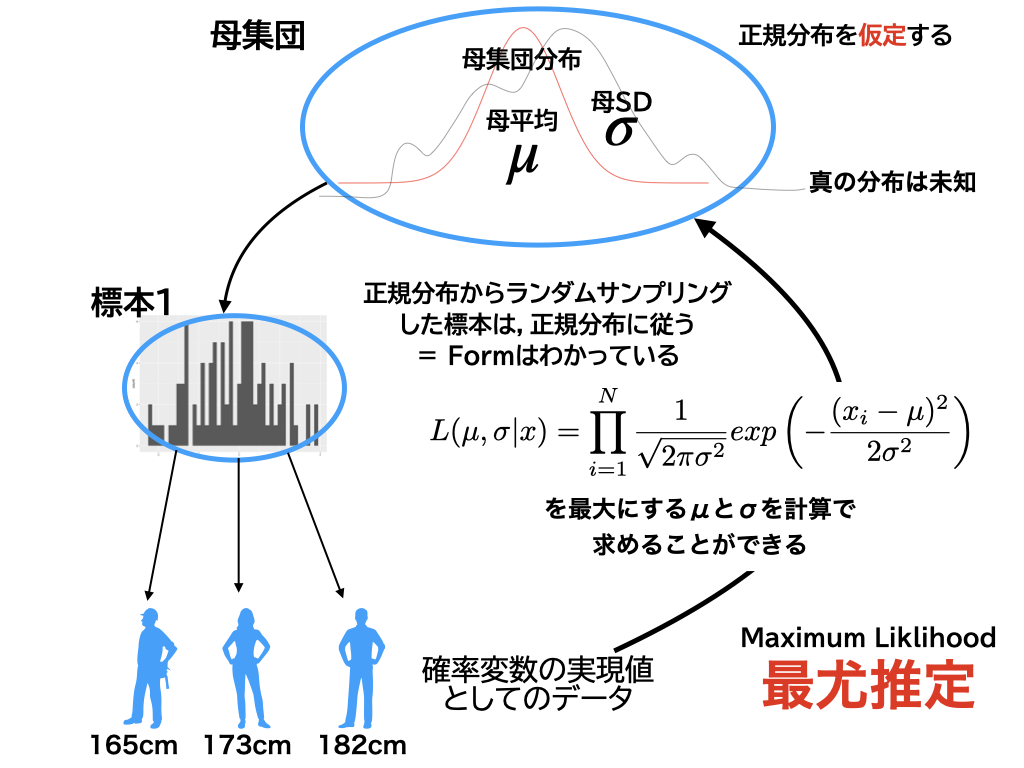
\includegraphics[keepaspectratio,width=0.8\linewidth]{figures/25_bayesian_intro/method2_ml.png}
	\caption{最尤法による母数の推定}
	\label{fig:25_03}
\end{figure}
これは母集団--標本の考え方からいっても非常に素直な発想です。いわば，確率分布をデータ生成機と考え，このデータを生み出す機械の設定(=パラメータ)はどうなっているんだろう，と考えるというわけです。手元のデータが最も再現されやすいところがその設定値だろうと考える，というわけですね。

この最尤法による推定も長く広く使われています。計算にもそれほど時間がかかるわけでもないですから，多くのデータを扱った推定法としてはスタンダードな手法です。この方法が確率モデルの基本中の基本，王道といってもいいかもしれません。実際，回帰分析をはじめとする線型モデルをはじめ，多くの統計モデルが最尤法を使って解を出しています。

サンプルサイズが小さく，平均値の差を検出することだけが目的なのであれば，モーメント法による検定が有効なのですが，平均値の差に「個体差」「条件差」といった要素が絡んでくるとか，正規分布しないデータ(カウントデータや比率のデータなど)を扱う場合，つまり一般化線型モデル，一般化線型混合モデルのような場合は，最尤法を用いることになります。かつては正規分布の平均値差モデルに合わせるために，データを変換して正規分布に近づけるというようなことがありましたが，今では正規分布に従わないデータをそのまま扱えるようになっています。

ただし，最尤法は確率の仮定とモデルが全面的に出てきますので，サンプルサイズが小さいと，推定値が不安定になったり，そもそも答えが出せなかったりすることがあります。もちろん確率分布の仮定が間違っている(比率のデータに正規分布を当てはめるなど)場合は適切な答えが得られません。そもそも，確率・尤度の考え方がちょっと難しいので，誤解なくしっかり理解しておくことが重要です。

\paragraph{ベイズ法}
そして第3の手法，ベイズ法です(図\ref{fig:25_05})。このベイズ法の原理となる定理そのものは18世紀に考えられていたものですが，近年の計算機科学の発展によって実用可能なものになり，一気にその利用が広がっています。
\begin{figure}[ht]
	\centering
	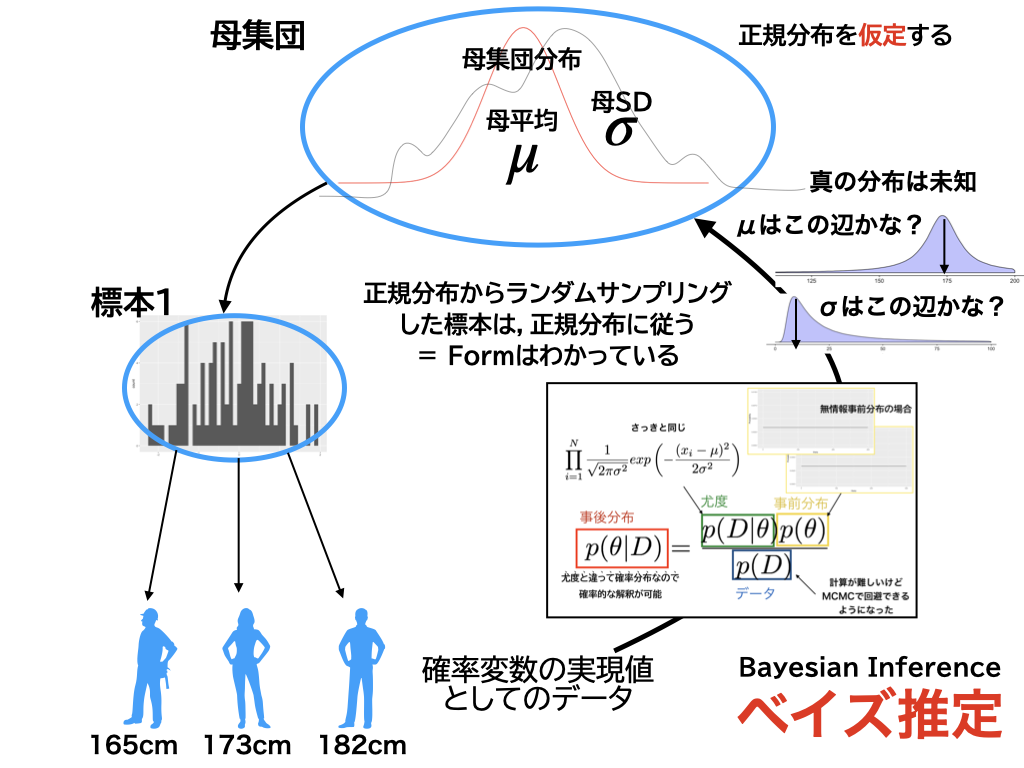
\includegraphics[keepaspectratio,width=0.8\linewidth]{figures/25_bayesian_intro/method3_bayes.png}
	\caption{ベイズ法による母数の推定}
	\label{fig:25_05}
\end{figure}

この方法を使うと，最尤法でうまく答えが出せなかったような複雑なモデルであっても，問題なく答えが出せます。最尤法の場合はたくさんのデータがないと安定した答えが出ない，というようなことがあるのですが，ベイズ法の場合は少ないデータであっても答えを出してくれます。ベイジアン\footnote{ベイズ統計学をする人，ベイズ流の，というのをベイジアンといいます。ちなみにコンピュータ言語Pythonを使う人はパイソニアン，組版ソフト\LaTeX を使う人はテフニシャンなどといった呼称があります。なぜかRを使う人は「Rおじさん」と言われています。}にとっての限界は，その人の想像力だけだ，という人もいるぐらいです\parencite{Lee201709}。

図にはベイズの結果の出し方，つまり事後の「確率分布」としての推定結果も示されています。モーメント法や最尤法は，推定値は一つの値でした。これに対してベイズ法は，結果が分布で出てきます。確率分布です。ですから，「この辺りにありそう」という感じ全体が答えになるのです。一つの値として得られないところが不思議に思えるかもしれません。この点，ベイズ法の結果の解釈が従来の方法(モーメント法・最尤法)と大きく違うところであり，ベイズ法の結果を解釈する上で重要なポイントです。根本的には先ほど述べたように，「母数は確率的に分布している」と考える(あるいは「母数は定数であるが，その値は確率的にしかわからない」と考える)という根本的な発想の転換を必要とするのです。

さて，三つの異なる手法を比較してきましたが，共通する点は「母集団に確率分布の仮定を置く」ということです。この仮定が間違っていれば，どの手法でやっても適切な推定にはなりません。そもそも推測統計学の根本問題として，少数のヒントから未知の答えを追い求めるという，不可能な条件設定での問題を解いていたわけですから，どれが正しいとか間違っているか，と言ったことを一概に言うことすらできません。しかし，仮定が適切であれば，どの手法を使っても同じ母集団についての推定なのですから，結果に大きな違いが出るわけではありません。モーメント法を使って有意にならなかったので，ベイズ法でなんとかならないか，というような考え方はお門違いで，厳に慎むべきです。

どの手法が良い悪いというのがあるわけではなく，考え方や特徴が異なるので，われわれユーザとしてはその手法の背景を理解し，異なる手法を用いる人との相互理解をするために，こうした違いに自覚的で言語化できるようにしておく必要があるでしょう。

\paragraph{ベイズ法の強み}

最尤法はサンプルサイズが大きくないと，安定した推定値が得られないことがあります。ベイズ法は，サンプルサイズが小さくても，モデルが複雑になっても答えが出せます。どうしてでしょうか？実践的には計算機科学の技術革新があったから，というのが答えなのですが(この点は第\ref{ch29_bayesianModeling}章で改めて扱います)，原理的なところからも説明しておきましょう。

まずもう一度ベイズの定理を見てみます。

\[ P(A|B) = \frac{P(B|A)P(A)}{P(B)} \]

ここで$P(A|B)$は事後確率，$P(B|A)$は尤度，$P(A)$は事前確率，$P(B)$は正規化定数と考えることができます。事前・事後確率は，そのまま事前分布・事後分布と，確率分布と言ってもいいでしょう\footnote{ここまでの説明では，離散的な変数による事前・事後確率でしたが，連続的な確率変数でも同様に扱うことができます。足し算が積分に変わると言ったことはありますが，ベイズの定理は同様に成り立ちます。}。つまり，

\[ \text{事後分布}　= \frac{\text{尤度} \times \text{事前分布}}{\text{正規化定数}} \]

という形です。
さて，最尤法はこの尤度だけを使って答えを出すのですが，ベイズ法の答え＝事後分布は，尤度に事前分布をかけています。この事前分布，つまり事前の情報や信念が，答えを出すために追加されているヒントなのです。このヒントのおかげで，尤度だけの最尤法では答えがでなくとも，ベイズ法では答えが出せる，ということになります。

次回は，ベイズ推定を実践的にどのように使うかを見ていきます。

\section{課題}
ある大学のクラスに，文系学部の学生が30人，理系学部の学生が20人います。統計の授業を履修済みの者は，文系に12人，理系に14人いました。このデータに基づいて，次の問いに答えなさい。
\paragraph{同時確率と周辺確率}このクラスから無作為に1人を選んだとき，「理系学部かつ履修済み」である\textbf{同時確率}はいくつでしょう。また，「履修済み」である\textbf{周辺確率}はいくつでしょう。
\paragraph{条件つき確率}選ばれた学生が履修済みであることが先に分かっているとき，その学生が理系学部である\textbf{条件つき確率}はいくつでしょう。またこれは「理系学部の学生が履修済みである確率」と一致しません。それはなぜでしょうか。
\paragraph{事前確率を使った推論}ある感染症の有病率は0.5\%，感染している人が検査で陽性となる確率は95\%，感染していない人が誤って陽性となる確率は5\%だとします。検査で陽性になった人が実際に感染している確率を求めましょう。
\paragraph{事前確率が変わると}前の問いと同じ検査を，有病率が10\%の集団で行ったとします。陽性になった人が実際に感染している確率はいくつになるでしょう。前の問いの答えと比べて，どのようなことが言えるでしょうか。

\section{補遺: ベイズの定理を使った推論の例}

ベイズの定理を使うとどういうことがわかるのでしょうか。
事前の確率が事後の確率に変換される，つまり推論情報のアップデートができることの数学的な意味はわかったとして，実際どのようなシーンで活用できるのでしょうか。
ここでは2つの例を見てみましょう。

\subsection{事前情報を活用しよう}
事前確率があることで何がわかるかについて，疫病の診断を例に考えてみたいと思います。

コロナウイルスに感染しているかどうかは，PCR検査で明らかになりますが，これらの検査の結果というのも確率的な要素があるのはご存知でしょうか。本当は感染していないのに，検査では陽性になってしまう，ということがゼロではありません。こういうのを\keyterm{偽陽性}{ぎようせい}{false positive}といいます。逆に感染しているのに，検査で検出できずに陰性になる，\keyterm{偽陰性}{ぎいんせい}{false negative}ということもあります。いずれも確率的な話です\footnote{勘のいい人はお気づきかもしれませんが，これは検定における2種類の間違い($\to$ セクション\ref{TypeI_II_Error}，Pp.\pageref{TypeI_II_Error})と同じ話であり，偽陽性は\keytermL{タイプ1エラー}{たいぷ1えらー}，偽陰性は\keytermL{タイプ2エラー}{たいぷ2えらー}のことです。有意水準は偽陽性率(本当は差がないのに差があると言ってしまう，本当は感染していないのに感染していると言ってしまう，せっかちなミス)として導入されていたのでした。}。

コロナに感染している$\to$検査で陽性になる，というのが因果関係ですが，我々は実際には検査で陽性である$\to$コロナに感染しているかもしれない，というように推論します。これを今日学んだ確率の言葉で書いてみましょう。

感染している状態で，陽性反応が出るというのは条件つき確率として表現できますね。$P(\mbox{陽性}|\mbox{感染})$，というわけです。さてここに，そもそもの感染率というのが別途見積もれたとします。$P(\mbox{感染})$ですね。さらにもうひとつ。感染しているかどうかに関係なく，陽性であるという結果だけ取り上げて$P(\mbox{陽性})$を考えることもできます。これが揃うと，先ほどの定理を使って
\[ \frac{P(\mbox{陽性}|\mbox{感染})P(\mbox{感染})}{P(\mbox{陽性})} = P(\mbox{感染}|\mbox{陽性})\]
を計算できます。つまり陽性になったという結果から，本当にかかっているかどうかの確率を計算できるのです。

多くの場合，検査で陽性だったら「もうだめだー」と思ってしまいがちです。これは陽性であると確実に検出できる，偽陽性がゼロの検査であれば正しい判断です。が，実際には確率的に判断すべき問題です。具体的に数字を例にして考えてみましょう。

ここでは乳がん検査(マンモグラフィー)の数値例でお話しします\footnote{乳がんについては古くからの疫学的知見で，大体の罹患率が事前情報としてあるからです。コロナについては流行の状況によって罹患率が大きく変動するので，事前確率を1つに定めることが難しいのです。}。
\begin{itemize}
	\item 40歳の女性が乳がんにかかる確率は1\%です。
	\item 乳がんである人が乳房X線検査で陽性と出る確率は90\%です。
	\item 本当は乳がんでなくても，検査で陽性と出る確率は8\%にすぎません。
	\item あなたが40歳の女性で検査結果が陽性だったとしたら，あなたが乳がんである確率はどれぐらいでしょうか。
\end{itemize}
これは先ほどの公式に当てはめて考えると，
\[\frac{0.9\times0.01}{0.9\times0.01+0.08\times0.99}=0.102 \]

となり，10\%ちょっとだということになります\footnote{おっと，計算についていけないぞ！と思った人。大丈夫です，いい方法があります。確率の計算は小数点を含みますし相対的な度数なのでわかりにくいですから，絶対的な度数に戻して考えればいいのです。たとえば10000人の世界だとして考えると，乳がんの人は1\%=100人です。乳がんでない人は9900人です。陽性になる人は乳がんで陽性反応が出るひと($100\times0.9=90$)と乳がんじゃないのに陽性反応が出る人($9900\times0.08=792$)の和で，882人です。陽性反応が出た人の中で本当に乳がんであるひとは，$90/882=0.102$となります。}。ずいぶんと印象が変わりますよね。PCR検査を複数回行うのは，これと同じような背景があるからです。

このように，事前確率があると，そこから遡って「診断された人が病気である確率」の計算をできるのです。逆確率，という言葉の意味が少しおわかりいただけたでしょうか。

\subsection{モンティ・ホール問題}

次は\keytermL{モンティ・ホール問題}{もんてぃほーるもんだい}という，有名な事例を取り上げます。モンティ・ホールというのは人名で，この人がテレビショー「Let's make a deal」の司会をしていたのですが，その中で行われたゲームに由来するお話しです。問題はこんな内容です。

\begin{quotation}
	プレーヤーの前に閉じた3つのドアがあって，1つのドアの後ろには景品の新車が，2つのドアの後ろには，はずれを意味するヤギがいる。プレーヤーは新車のドアを当てると新車がもらえる。プレーヤーが1つのドアを選択した後，司会のモンティが残りのドアのうちヤギがいるドアを開けてヤギを見せる。

	ここでプレーヤーは，最初に選んだドアを，残っている開けられていないドアに変更してもよいと言われる。
	ここでプレーヤーはドアを変更すべきだろうか？
\end{quotation}

直感的には，選択したドアを変えても変えなくても，新車が得られる確率は1/3で変わらない，と思いますよね。でも実際は，変えた方が当たる確率は2倍になるのです。

なんでそんなことになるのか，と思うかもしれません。変えても変えなくても，確率は変わらないじゃないか，と思うのではないでしょうか。

実は明文化されていませんが，この話のポイントは，司会者のモンティは答えを知っていて，テレビ番組を盛り上げるために，\underline{必ずヤギ(ハズレ)のドアを開ける}ということです。司会者が「じゃあこっちを開けてみましょう，わー新車だ。ザンネーン」といったらシラけてしまうからですね。司会者がハズレのドアを開けるということは，新しい情報が追加されているということでもあります。であれば私たちは，情報をアップデートできるはずであり，確信度は変わるはずです。

3つのドアをA,B,Cとして，どこかに当たりが入っているのですが，確信度はどれも同じぐらいなので，それぞれ1/3の確率だと考えます。
あなたがAのドアを選んだとします。当たっている確率は1/3です。BかCが当たっている確率は，Aではないので，2/3になります。
モンティはどのドアを開けるでしょうか？Aのドアは番組がしらけてしまうので開けません。BかCを開けるしかないのです。ここでもし，ドアBの後ろに新車があるとモンティはこれを開けられないので，ドアCが開けられることになります。そうすると当然，ヤギが出てくることになりますね。さて，これまでBかCがあたりの確率は2/3でした。でもCがあたりということはあり得ないので，この2/3の確率はB=2/3,C=0にアップデートされるはずです。
あなたが最初に選んだAのドアは，1/3の確率だったわけですから，「AからBに変えますか？」と言われると，変えた方が2倍得だ(A=1/3,B=2/3,C=0)ということになります。

これはたとえば，3つのドアでなくて100枚のドアがある場合で考えてみると，わかりやすいかもしれません。100枚のドアがあって，あなたが1番目のドアを選び，モンティが100，99，98，...，5，4，3番目のドア，と順番にドアを開け続けて，すべてにヤギが入っていたとします。それでも2番目のドアに変えないか？といわれると・・・モンティはどうして残り99枚のどれを開けてもよかったのに，隣のドアを開けなかったのか？と思いますよね。

モンティ・ホール問題は他にもいろいろな説明の仕方があります。納得いかなかった人は，Wikipediaなどで調べてみると良いでしょう。

くどいようですが，ポイントは「情報がもたらされたときに，確率はアップデートできる」というところにあります。事前確率ともたらされる情報をつかって，確信度をどんどんアップデートしていく，これがベイズ法の考え方なのです。


\end{document}
